\section{计算张量网络的梯度}\label{chapter:gradients}
在一般情形下优化张量网络，是许多研究领域共同面临的重大挑战。针对矩阵的优化技术虽已发展良多，但把这些方法推广到张量网络仍然不易~\citep{liao2019differentiable}。其困难源于张量收缩的高昂计算代价，也源于高维情形缺少高效的优化算法。此外，只要张量网络的结构略微复杂，手工用链式法则求梯度便令人却步。本章介绍一种优雅而直观的方法：借助张量网络的图示记法来推导高阶导数。该方法表明，张量网络函数的导数往往继承初始张量网络的低秩结构。

下一节先针对以向量为输入的函数，给出梯度与雅可比矩阵（Jacobian）的经典概念，再把它们推广到以张量为输入、以张量为输出的函数。
\subsection{雅可比矩阵}
我们先回顾定义在 $\mathbb{R}^n$ 上的函数的梯度与雅可比矩阵这两个经典概念。

\begin{definition}
  设 $f:\RR^n\to\RR$ 与 $g:\RR^n\to\RR^p$。$f$ 的梯度与 $g$ 在 $\theta\in\mathbb{R}^n$ 处的雅可比矩阵定义为
    $$\nabla_\theta f = \left[\frac{\partial f(\theta)}
{\partial\theta_1},\frac{\partial f(\theta)}{\partial\theta_2},\dots,\frac{\partial f(\theta)} 
    {\partial\theta_n}\right]^\ts
        =
    \begin{tikzpicture}[baseline=\baseline]
    \tikzset{tensor/.style = {minimum size = 0.5cm,shape = circle,thick,draw=black,inner sep = 0pt}, edge/.style   = {thick,line width=.4mm}}
    \def\y{0}
     \def\x{0}
    \node[tensor,fill=blue!40!red!60!white] (a1) at (\x,\y){};
    \draw[edge](a1) -- (\x+0.75,\y)node [midway, above]{\edgelabel{$n$}};
    \end{tikzpicture} \in\mathbb{R}^n,$$
    以及
    $$\frac{\partial g(\theta)}{\partial\theta} = \left(\frac{\partial g(\theta)_i}{\partial\theta_j}\right)_{i=1,\cdots,p\atop j=1,\cdots, n}
    =
    \begin{tikzpicture}[baseline=\baseline]
    \tikzset{tensor/.style = {minimum size = 0.5cm,shape = circle,thick,draw=black,inner sep = 0pt}, edge/.style   = {thick,line width=.4mm}}
    \def\y{0}
     \def\x{0}
    \node[tensor,fill=blue!20!red!50!white] (A) at (\x,\y){};
    \draw[edge](A) -- (\x+0.75,\y)node [midway, above]{\scalebox{0.7}{\dimcolor{$n$}}};
    \draw[edge](A) -- (\x-0.75,\y)node [midway, above]{\scalebox{0.7}{\dimcolor{$p$}}};
    \end{tikzpicture}\in\mathbb{R}^{p\times n}.$$  
\end{definition}
雅可比矩阵的概念可以自然推广到以张量为输入、输出张量（阶数任意）的函数。

\begin{definition}
 设 $f:\RR^{n_1\times\dots\times n_N}\to\RR^{m_1\times\dots\times m_M}$，。$f$ 在 $\theta\in\RR^{n_1\times\dots\times n_N}$ 处的\emph{雅可比张量}是张量 $\frac{\partial f}{\partial\theta}\in\RR^{m_1\times\dots\times m_M\times n_1\times\dots\times n_N}$
 定义为
\begin{align*}
   \frac{\partial f(\theta)}{\partial\theta} 
   &= 
   \left(\frac{\partial f(\theta)_{i_1,\dots,i_M}}{\partial\theta_{j_1,\dots,j_N}}\right)_{i_1\in[m_1],\cdots,i_M\in[m_M]\atop j_1\in[n_1],\cdots,j_N
\in[n_N]}\\
&=
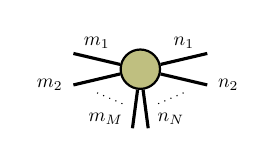
\begin{tikzpicture}[baseline=-0.5ex]
    \tikzset{tensor/.style = {minimum size = 0.5cm,shape = circle,thick,draw=black,inner sep = 0pt}, edge/.style = {thick,line width=.4mm},every loop/.style={}}
    \def\x{6}
    \node[tensor,fill=green!50!red!50!white] (T) at (\x,0) {};
    \draw[edge] (T) -- (\x-0.85,0.2)node [midway, above]{\scalebox{0.7}{\dimcolor{$m_1$}}};
    \draw[edge] (T) -- (\x-0.85,-0.2)node [left]{\scalebox{0.7}{\dimcolor{$m_2$}}};
    \draw[edge] (T) -- (\x-0.1,-0.75)node [near end, left]{\scalebox{0.7}{\dimcolor{$m_M$}}};
    \draw[dotted] (\x-0.55,-0.3) -- (\x-0.2,-0.45);
    \draw[edge] (T) -- (\x+0.85,0.2)node [midway, above]{\scalebox{0.7}{\dimcolor{$n_1$}}};
    \draw[edge] (T) -- (\x+0.85,-0.2)node [right]{\scalebox{0.7}{\dimcolor{$n_2$}}};
    \draw[edge] (T) -- (\x+0.1,-0.75)node [near end, right]{\scalebox{0.7}{\dimcolor{$n_N$}}};
    \draw[dotted] (\x+0.55,-0.3) -- (\x+0.2,-0.45);
    \end{tikzpicture}\in\RR^{m_1\times\cdots\times m_M\times n_1\times\cdots\times n_N}. 
\end{align*}
\end{definition}




下面的定理表明，张量网络关于某个核心张量的一阶导数，用张量网络本身就能轻松算出。

\begin{theorem}\label{thm:gradients}
    设 $\Tt$ 是由张量网络给出的张量，其中 $\Gt$ 是在该张量网络中\emph{只出现一次}的核心张量。那么，把 $\Gt$ 从 $\Tt$ 的张量网络中移除，所得即 $\frac{\partial \Tt}{\partial \Gt}$。 
\end{theorem}
下面的例子说明如何将定理~\ref{thm:gradients}用于张量网络。
\paragraph{示例}
设 
$\begin{tikzpicture}[baseline=\baseline]
    \tikzset{tensor/.style = {minimum size = 0.5cm,shape = circle,thick,draw=black,inner sep = 0pt}, edge/.style = {thick,line width=.4mm},every loop/.style={}}
    \def\x{0}
    \def\y{0}
     \node[tensor,fill=green!50!red!50!white] (B) at (\x+1,\y) {$\Xt$};
    \draw[edge] (B) -- (\x+0.25,0) node [midway,above] {\scalebox{0.7}{\dimcolor{$d_1$}}};
    \draw[edge] (B) -- (\x+1.85,\y) node [midway,above] {\scalebox{0.7}{\dimcolor{$d_3$}}};
    \draw[edge] (B) -- (\x+1,\y-0.85) node [midway,left] {\scalebox{0.7}{\dimcolor{$d_2$}}};
\end{tikzpicture}
=
\begin{tikzpicture}[baseline=\baseline]
    \tikzset{tensor/.style = {minimum size = 0.5cm,shape = circle,thick,draw=black,inner sep = 0pt}, edge/.style = {thick,line width=.4mm},every loop/.style={}}
    \def\x{0}
    \def\y{0}
    \node[tensor,fill=red!30!white] (A) at (\x+2,\y) {$\Gt_1$};
    \node[tensor,fill=red!50!white] (B) at (\x+3.2,\y) {$\Gt_2$};
    \node[tensor,fill=blue!30!white] (C) at (\x+2.6,\y-0.7) {$\Gt_3$};
    \node[tensor,fill=blue!50!white] (D) at (\x+4.3,\y) {$\Gt_4$};
    \draw[edge] (A) -- (B) node [midway,above] {\scalebox{0.7}{\dimcolor{$R_1$}}};
    \draw[edge] (A) -- (C);
    \node[draw=none] () at (\x+2,\y-0.5) {\scalebox{0.7}{\dimcolor{$R_2$}}};
    \draw[edge] (B) -- (C);
    \node[draw=none] () at (\x+3.2,\y-0.5) {\scalebox{0.7}{\dimcolor{$R_3$}}};
    \draw[edge] (B) -- (D) node [midway,above] {\scalebox{0.7}{\dimcolor{$R_4$}}};
    \draw[edge] (A) -- (\x+2,\y+0.7) node [midway,left] {\scalebox{0.7}{\dimcolor{$d_1$}}};
    \draw[edge] (D) -- (\x+4.3,\y+0.7) node [midway,right] {\scalebox{0.7}{\dimcolor{$d_3$}}};
    \draw[edge] (C) -- (\x+2.6,\y-1.5) node [midway,left] {\scalebox{0.7}{\dimcolor{$d_2$}}};
\end{tikzpicture}
$ 为张量网络。注意，可以把 $\Xt$ 看作其张量网络表示中任一核心张量的函数，于是自然会问：$\Xt$ 关于例如 $\Gt_2$ 或 $\Gt_4$ 的雅可比矩阵是什么。
上述定理给出了计算这些导数的简便途径：
\begin{itemize}
\item 根据定理~\ref{thm:gradients}，要求 $\Xt$ 关于 $\Gt_2$ 的梯度，需从张量网络中移除核心张量 $\Gt_2$，即
$$
\frac{\partial}{\partial\Gt_2}\left(\begin{tikzpicture}[baseline=\baseline]
    \tikzset{tensor/.style = {minimum size = 0.5cm,shape = circle,thick,draw=black,inner sep = 0pt}, edge/.style = {thick,line width=.4mm},every loop/.style={}}
    \def\y{0}
    \def\x{0}
    \node[tensor,fill=red!30!white] (A) at (\x+2,\y) {$\Gt_1$};
    \node[tensor,fill=red!50!white] (B) at (\x+3.2,\y) {$\Gt_2$};
    \node[tensor,fill=blue!30!white] (C) at (\x+2.6,\y-0.7) {$\Gt_3$};
    \node[tensor,fill=blue!50!white] (D) at (\x+4.3,\y) {$\Gt_4$};
    \draw[edge] (A) -- (B) node [midway,above] {\scalebox{0.7}{\dimcolor{$R_1$}}};
    \draw[edge] (A) -- (C);
    \node[draw=none] () at (\x+2,\y-0.5) {\scalebox{0.7}{\dimcolor{$R_2$}}};
    \draw[edge] (B) -- (C);
    \node[draw=none] () at (\x+3.2,\y-0.5) {\scalebox{0.7}{\dimcolor{$R_3$}}};
    \draw[edge] (B) -- (D) node [midway,above] {\scalebox{0.7}{\dimcolor{$R_4$}}};
    \draw[edge] (A) -- (\x+2,\y+0.7) node [midway,left] {\scalebox{0.7}{\dimcolor{$d_1$}}};
    \draw[edge] (D) -- (\x+4.3,\y+0.7) node [midway,right] {\scalebox{0.7}{\dimcolor{$d_3$}}};
    \draw[edge] (C) -- (\x+2.6,\y-1.5) node [midway,left] {\scalebox{0.7}{\dimcolor{$d_2$}}};
    \end{tikzpicture}\right)
=
    \begin{tikzpicture}[baseline=\baseline]
    \tikzset{tensor/.style = {minimum size = 0.5cm,shape = circle,thick,draw=black,inner sep = 0pt}, edge/.style = {thick,line width=.4mm},every loop/.style={}}
    \def\y{-0.5}
    \def\x{0}
    \node[tensor,fill=red!30!white] (A) at (\x,\y+1) {$\Gt_1$};
    \node[tensor,fill=blue!30!white] (C) at (\x+0.6,\y+0.2) {$\Gt_3$};
    \node[tensor,fill=blue!50!white] (D) at (\x+2,\y+0.5) {$\Gt_4$};
    \draw[edge] (A) -- (C);
    \draw[edge] (A) -- (\x,\y+1.7) node [midway,left] {\scalebox{0.7}{\dimcolor{$d_1$}}};
    \draw[edge] (A) -- (\x+0.7,\y+1) node [midway,above] 
{\scalebox{0.7}{\dimcolor{$R_1$}}};
    \draw[edge] (D) -- (\x+3,\y+0.5) node [midway,above] {\scalebox{0.7}{\dimcolor{$R_4$}}};
    \draw[edge] (C) -- (\x+0.6,\y-0.7) node [midway,left] {\scalebox{0.7}{\dimcolor{$d_2$}}};
    \draw[edge] (C) -- (\x+1.3,\y+0.2) node [midway,above] {\scalebox{0.7}{\dimcolor{$R_3$}}};
    \draw[edge] (D) -- (\x+2,\y+1.3) node [midway,left] {\scalebox{0.7}{\dimcolor{$d_3$}}};
    \node[draw=none] () at (\x,\y+0.4) {\scalebox{0.7}{\dimcolor{$R_2$}}};
\end{tikzpicture}.
$$ 
要理解这一做法为何成立，可把 $\Xt$ 的张量分解看作矩阵-向量乘积：
$$
\Mb\vb 
=
\begin{tikzpicture}[baseline=\baseline]
    \tikzset{tensor/.style = {minimum size = 0.5cm,shape = circle,thick,draw=black,inner sep = 0pt}, edge/.style = {thick,line width=.4mm},every loop/.style={}}
    \def\y{1}
    \def\x{0}
     \node[tensor,fill=red!30!white](G_1) at (\x,\y) {$\Gt_1$};
    \node[tensor,fill=blue!30!white] (G_3) at (\x,\y-1) {$\Gt_3$};
     \node[tensor,fill=red!50!white](G_2) at (\x+2,\y-1) {$\Gt_2$};
    \node[tensor,fill=blue!50!white] (G_4) at (\x,\y-2) {$\Gt_4$};
    \node[tensor,fill=red!50!white] (G_2) at (\x+2,\y-1) {$\Gt_2$};
    \draw[edge](G_1) -- (\x-1,\y) -- (\x-1,\y-0.85) -- (\x-1.75,\y-0.85);
    \draw[edge](G_3)-- (\x-1.75,\y-1)node [left] {\scalebox{0.7}{\dimcolor{$d_1d_2d_3$}}};
    \draw[edge](G_2)--(G_1)node [midway,above] {\scalebox{0.7}{\dimcolor{$R_1$}}};
    \draw[edge](G_2)--(G_3)node [midway,above] {\scalebox{0.7}{\dimcolor{$R_3$}}};
    \draw[edge](G_1)--(G_3)node [midway,left] {\scalebox{0.7}{\dimcolor{$R_2$}}};
    \draw[edge](G_2)--(G_4)node [midway,above] {\scalebox{0.7}{\dimcolor{$R_4$}}};
    \draw[edge] (G_4) -- (\x-1,\y-2) -- (\x-1,\y-1.15) -- (\x-1.75,\y-1.15);
    \draw[dotted] (\x+0.45,\y+0.65) -- (\x+0.45,\y-2.35);
\end{tikzpicture},
$$
其中 $\vb = \vectorize(\Gt_2) $，而 $\Mb$ 是把张量网络余下部分矩阵化后得到的矩阵。 
利用线性映射的雅可比矩阵这一经典恒等式，便得到期望的结果：
$$\frac{\partial\Mb\vb}{\partial\vb} = \Mb = 
\begin{tikzpicture}[baseline=\baseline]
    \tikzset{tensor/.style = {minimum size = 0.5cm,shape = circle,thick,draw=black,inner sep = 0pt}, edge/.style = {thick,line width=.4mm},every loop/.style={}}
    \def\y{1}
    \def\x{0}
     \node[tensor,fill=red!30!white](G_1) at (\x,\y) {$\Gt_1$};
    \node[tensor,fill=blue!30!white] (G_3) at (\x,\y-1) {$\Gt_3$};
    \node[tensor,fill=blue!50!white] (G_4) at (\x,\y-2) {$\Gt_4$};
    \draw[edge](G_1) -- (\x-0.85,\y) -- (\x-0.85,\y-0.9) -- (\x-1.5,\y-0.9);
    \draw[edge](G_3)-- (\x-1.5,\y-1)node [left] {\scalebox{0.7}{\dimcolor{$d_1d_2d_3$}}};
    \draw[edge](G_1)-- (\x+0.85,\y) -- (\x+0.85,\y-0.9) -- (\x+1.5,\y-0.9);
    \draw[edge](G_3) -- (\x+1.5,\y-1) node [right] {\scalebox{0.7}{\dimcolor{$R_1R_3R_4$}}};
    \draw[edge](G_1)--(G_3)node [midway,left] {\scalebox{0.7}{\dimcolor{$R_2$}}};
    \draw[edge] (G_4) -- (\x+0.85,\y-2) -- (\x+0.85,\y-1.1) -- (\x+1.5,\y-1.1);
    \draw[edge] (G_4) -- (\x-0.85,\y-2) -- (\x-0.85,\y-1.1) -- (\x-1.5,\y-1.1);
\end{tikzpicture}\in\RR^{d_1d_2d_3\times R_1R_3R_4}.
$$
\item 根据定理~\ref{thm:gradients}，要求 $\Xt$ 关于 $\Gt_4$ 的梯度，需从相应的张量网络中移除核心张量 $\Gt_4$。即 
$$
    \frac{\partial}{\partial\Gt_4}\left(\begin{tikzpicture}[baseline=\baseline]
    \tikzset{tensor/.style = {minimum size = 0.5cm,shape = circle,thick,draw=black,inner sep = 0pt}, edge/.style = {thick,line width=.4mm},every loop/.style={}}
    \def\x{0}
    \def\y{0}
    \node[tensor,fill=red!30!white] (A) at (\x+2,\y) {$\Gt_1$};
    \node[tensor,fill=red!50!white] (B) at (\x+3.2,\y) {$\Gt_2$};
    \node[tensor,fill=blue!30!white] (C) at (\x+2.6,\y-0.7) {$\Gt_3$};
    \node[tensor,fill=blue!50!white] (D) at (\x+4.3,\y) {$\Gt_4$};
    \draw[edge] (A) -- (B) node [midway,above] {\scalebox{0.7}{\dimcolor{$R_1$}}};
    \draw[edge] (A) -- (C);
    \node[draw=none] () at (\x+2,\y-0.5) {\scalebox{0.7}{\dimcolor{$R_2$}}};
    \draw[edge] (B) -- (C);
    \node[draw=none] () at (\x+3.2,\y-0.5) {\scalebox{0.7}{\dimcolor{$R_3$}}};
    \draw[edge] (B) -- (D) node [midway,above] {\scalebox{0.7}{\dimcolor{$R_4$}}};
    \draw[edge] (A) -- (\x+2,\y+0.7) node [midway,left] {\scalebox{0.7}{\dimcolor{$d_1$}}};
    \draw[edge] (D) -- (\x+4.3,\y+0.7) node [midway,right] {\scalebox{0.7}{\dimcolor{$d_3$}}};
    \draw[edge] (C) -- (\x+2.6,\y-1.5) node [midway,left] {\scalebox{0.7}{\dimcolor{$d_2$}}};
    \end{tikzpicture}\right)
=
    \begin{tikzpicture}[baseline=\baseline]
    \tikzset{tensor/.style = {minimum size = 0.5cm,shape = circle,thick,draw=black,inner sep = 0pt}, edge/.style = {thick,line width=.4mm},every loop/.style={}}
    \def\y{-0.5}
    \def\x{0}
    \node[tensor,fill=red!30!white] (A) at (\x+2,\y+1) {$\Gt_1$};
    \node[tensor,fill=red!50!white] (B) at (\x+3.2,\y+1) {$\Gt_2$};
    \node[tensor,fill=blue!30!white] (C) at (\x+2.6,\y) {$\Gt_3$};
    \draw[edge] (A) -- (B) node [midway,above] {\scalebox{0.7}{\dimcolor{$R_1$}}};
    \draw[edge] (A) -- (C);
    \node[draw=none] () at (\x+2,\y+0.5) {\scalebox{0.7}{\dimcolor{$R_2$}}};
    \draw[edge] (B) -- (C);
    \node[draw=none] () at (\x+3.2,\y+0.5) {\scalebox{0.7}{\dimcolor{$R_3$}}};
    \draw[edge] (B) -- (\x+4,\y+1) node [midway,above] {\scalebox{0.7}{\dimcolor{$R_4$}}};
    \draw[edge] (A) -- (\x+2,\y+1.7) node [midway,left] {\scalebox{0.7}{\dimcolor{$d_1$}}};
    \draw[edge] (C) -- (\x+2.6,\y-0.7) node [midway,left] {\scalebox{0.7}{\dimcolor{$d_2$}}};
    \draw[edge] (\x+4.5,\y+1) -- (\x+4.5,\y+1.65) node [midway,right] {\scalebox{0.7}{\dimcolor{$d_3$}}};
    \end{tikzpicture}.
$$
注意 $\Gt_4$ 的悬空腿（dangling leg）仍留在雅可比张量中！为理解这一点，可再次把 $\Xt$ 的张量分解看作矩阵-向量乘积 $\Mb\vb$，使得 
$$
\Mb\vb = \begin{tikzpicture}[baseline=\baseline]
    \tikzset{tensor/.style = {minimum size = 0.5cm,shape = circle,thick,draw=black,inner sep = 0pt}, edge/.style = {thick,line width=.4mm},every loop/.style={}}
    \def\y{0.7}
    \def\x{0}
     \node[tensor,fill=red!30!white](G_1) at (\x,\y) {$\Gt_1$};
     \node[tensor,fill=red!50!white](G_2) at (\x+1,\y) {$\Gt_2$};
    \node[tensor,fill=blue!30!white] (G_3) at (\x+0.5,\y-1) {$\Gt_3$};
    \node[tensor,fill=blue!50!white] (G_4) at (\x+2.25,\y-1.5) {$\Gt_4$};
    \draw[edge](G_2)--(G_3);
    \draw[edge](G_1)--(G_2)node [midway,above] {\scalebox{0.7}{\dimcolor{$R_1$}}};
    \draw[edge](G_1)--(G_3);
    \draw[edge](G_2)--(G_4)node [midway,above=0.05cm] {\scalebox{0.7}{\dimcolor{$R_4$}}};
    \draw[edge](G_1) -- (\x,\y-1.35) -- (\x+0.35,\y-1.35) -- (\x+0.35,\y-2);
    \draw[edge](G_3)--(\x+0.5,\y-2)node [below] {\scalebox{0.7}{\dimcolor{$d_1d_2d_3$}}};
    \draw[edge](G_4) -- (\x+0.75,\y-1.5) -- (\x+0.75,\y-2);
    \draw[dotted] (\x+2.25,\y-0.75) -- (\x+1,\y-2);
\end{tikzpicture},
$$
此时 $\vb  =\vectorize(\Gt_4)$。
对该张量网络关于 $\vb = \vectorize(\Gb_4)$ 求导，便得到期望的结果：  $$\frac{\partial\Mb\vb}{\partial\vb} = \Mb
=
\begin{tikzpicture}[baseline=\baseline]
\tikzset{tensor/.style = {minimum size = 0.5cm,shape = circle,thick,draw=black,inner sep = 0pt}, edge/.style = {thick,line width=.4mm},every loop/.style={}}
    \def\y{1}
    \def\x{0}
     \node[tensor,fill=red!30!white](G_1) at (\x,\y) {$\Gt_1$};
     \node[tensor,fill=red!50!white](G_2) at (\x+1,\y) {$\Gt_2$};
    \node[tensor,fill=blue!30!white] (G_3) at (\x+0.5,\y-1) {$\Gt_3$};
    \draw[edge](G_2)--(G_3);
    \draw[edge](G_1)--(G_2)node [midway,above] {\scalebox{0.7}{\dimcolor{$R_1$}}};
    \draw[edge](G_1)--(G_3);
    \draw[edge](G_1) -- (\x,\y-1.35) -- (\x+0.35,\y-1.35) -- (\x+0.35,\y-2);
    \draw[edge](G_3)--(\x+0.5,\y-2)node [below] {\scalebox{0.7}{\dimcolor{$d_1d_2d_3$}}};
     \draw[edge](G_2) -- (\x+1.85,\y)node [midway, above] {\scalebox{0.7}{\dimcolor{$R_4$}}};
    \draw[edge](\x+1.85,\y-1.5) -- (\x+0.75,\y-1.5) -- (\x+0.75,\y-2);
\end{tikzpicture}\in\RR^{d_1d_2d_3\times R_4}.$$
注意，对某个张量求导只是从网络中移除相应的节点，而与它相连的边（腿）保持原样。
\end{itemize}
下面说明如何用定理~\ref{thm:gradients}不费力气地推出经典的导数与梯度计算式。 
\paragraph{用张量网络重新推导经典恒等式}
\begin{enumerate}
\item 
    $\frac{\partial\langle\ub,\vb\rangle}{\partial \ub}
=
    \frac{\partial\left(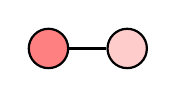
\begin{tikzpicture}[baseline=-0.1ex]
    \tikzset{tensor/.style = {minimum size = 0.5cm,shape = circle,thick,draw=black,inner sep = 0pt}, edge/.style = {thick,line width=.4mm},every loop/.style={}}
    \def\x{0}
    \def\y{0}
    \node[tensor,fill=red!50!white] (u) at (\x+1,\y) {$\ub$};
    \node[tensor,fill=red!20!white] (v) at (\x+2,\y) {$\vb$};
    \draw[edge] (u) -- (v);
    \end{tikzpicture}\right)}{\partial\left(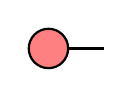
\begin{tikzpicture}[baseline=-0.1ex]
    \tikzset{tensor/.style = {minimum size = 0.5cm,shape = circle,thick,draw=black,inner sep = 0pt}, edge/.style = {thick,line width=.4mm},every loop/.style={}}
    \def\x{0}
    \def\y{0}
    \node[tensor,fill=red!50!white] (u) at (\x+1,\y) {$\ub$};
    \draw[edge] (u) -- (\x+1.7,\y);
    \end{tikzpicture}\right)}
=
    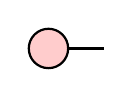
\begin{tikzpicture}[baseline=-0.1ex]
    \tikzset{tensor/.style = {minimum size = 0.5cm,shape = circle,thick,draw=black,inner sep = 0pt}, edge/.style = {thick,line width=.4mm},every loop/.style={}}
    \def\x{6}
    \def\y{0}
    \node[tensor,fill=red!20!white] (v) at (\x+2,\y) {$\vb$};
    \draw[edge] (v) -- (\x+2.7,\y);
    \end{tikzpicture}
    =
    \vb
    $
